\chapter{Cinétique complexe~: chaînes, enzymes et oscillations}\label{ch:b3:complex-kinetics}

Un bécher de solution agitée devient incolore, puis ambré, puis bleu,
puis de nouveau incolore, et recommence pendant de longues minutes~;
versé dans une boîte, le même mélange dessine des spirales qui tournent
et se propagent. Quand Boris Belousov décrivit une telle réaction en
1951, son manuscrit fut refusé~: un système chimique, pensait le
rapporteur, ne peut pas aller et venir, puisqu'il doit descendre vers
l'équilibre. Il descend bien~; simplement, il ne descend pas en ligne
droite. Ce chapitre traite des mécanismes à plusieurs étapes dont les
intermédiaires sont régénérés~: \omterm{def:b3:complex-kinetics:chain}{réactions en chaîne} et explosions,
molécules qui ont besoin de collisions pour se décomposer seules,
\omterm{def:b3:complex-kinetics:enzyme}{enzymes}, et \omterm{def:b3:complex-kinetics:oscillating}{réactions oscillantes}, avec les méthodes qui suivent des
réactions trop rapides pour être mélangées à la main.

\begin{recall}
Le volume de première année a défini un mécanisme réactionnel comme une
suite d'actes élémentaires, l'étape cinétiquement déterminante, les
approximations du pré-équilibre rapide et des états quasi stationnaires,
et les catalyseurs. Le volume de deuxième année a nommé les étapes d'une
chaîne radicalaire (amorçage, propagation, rupture), les amorceurs
radicalaires et la longueur de chaîne cinétique d'une polymérisation, et
a ajusté des droites par les moindres carrés. Le
\Cref{ch:b3:rate-theories} a donné la \omterm{def:b3:rate-theories:tst}{théorie de l'état de transition} et
la limite de diffusion, d'environ \qty{e10}{L.mol^{-1}.s^{-1}}.
\end{recall}

\section{Réactions en chaîne}

\begin{definition}[Réaction en chaîne, porteur de chaîne]\label{def:b3:complex-kinetics:chain}
Une \emph{réaction en chaîne}\index{reaction en chaine@réaction en chaîne} est une réaction dans
laquelle des intermédiaires réactifs, les \emph{porteurs de
chaîne}\index{porteur de chaine@porteur de chaîne}, sont régénérés par
un cycle d'étapes de propagation, de sorte qu'un seul événement
d'amorçage transforme de nombreuses molécules de réactif.
\end{definition}

Bodenstein mesura en 1906 la vitesse de $\ce{H2 + Br2 -> 2 HBr}$ et
trouva une loi qu'aucun acte unique ne pouvait produire~: la vitesse
croît comme $[\ce{Br2}]^{1/2}$ et diminue à mesure que HBr
s'accumule. Le mécanisme fut écrit en 1919~:
\begin{center}
\begin{tabular}{lll}
amorçage & $\ce{Br2 -> 2 Br}$ & $k_1$ \\
propagation & $\ce{Br + H2 -> HBr + H}$ & $k_2$ \\
propagation & $\ce{H + Br2 -> HBr + Br}$ & $k_3$ \\
inhibition & $\ce{H + HBr -> H2 + Br}$ & $k_4$ \\
rupture & $\ce{2 Br -> Br2}$ & $k_{-1}$
\end{tabular}
\end{center}
(les collisions avec un troisième corps M, qui apportent et emportent
l'énergie des étapes d'amorçage et de rupture, restent implicites).

\begin{theorem}[La loi de vitesse de la réaction dihydrogène--dibrome]\label{thm:b3:complex-kinetics:hbr}
Avec l'approximation des états quasi stationnaires pour Br et pour H,
la vitesse $v = \frac12\,\dd[\ce{HBr}]/\dd t$
du mécanisme vaut
\[
  v = \frac{k[\ce{H2}][\ce{Br2}]^{1/2}}{1 + k'[\ce{HBr}]/[\ce{Br2}]},
  \qquad k = k_2\Bigl(\frac{k_1}{k_{-1}}\Bigr)^{1/2},\ k' = \frac{k_4}{k_3}.
\]
\end{theorem}

\begin{proof}
AEQS pour H~: $k_2[\ce{Br}][\ce{H2}] = k_3[\ce{H}][\ce{Br2}] + k_4[\ce{H}][\ce{HBr}]$. AEQS pour Br~:
$2k_1[\ce{Br2}] - k_2[\ce{Br}][\ce{H2}] + k_3[\ce{H}][\ce{Br2}] + k_4[\ce{H}][\ce{HBr}] - 2k_{-1}[\ce{Br}]^2 = 0$.
En additionnant les deux
équations, les termes de propagation se compensent~: $k_1[\ce{Br2}] = k_{-1}[\ce{Br}]^2$, donc $[\ce{Br}] =
(k_1/k_{-1})^{1/2}[\ce{Br2}]^{1/2}$. Alors $[\ce{H}] = k_2[\ce{Br}][\ce{H2}]/(k_3[\ce{Br2}] + k_4[\ce{HBr}])$ et
\[
  \frac{\dd[\ce{HBr}]}{\dd t} = k_2[\ce{Br}][\ce{H2}] + k_3[\ce{H}][\ce{Br2}] - k_4[\ce{H}][\ce{HBr}] = 2k_3[\ce{H}][\ce{Br2}]
  = \frac{2k_2[\ce{Br}][\ce{H2}]}{1 + (k_4/k_3)[\ce{HBr}]/[\ce{Br2}]},
\]
en utilisant la première équation~; en substituant $[\ce{Br}]$, on obtient le résultat.
\end{proof}

\begin{omfigure}
\begin{tikzpicture}[font=\small, >=Stealth]
  \node[draw, circle, minimum size=9mm, omDef, thick] (br) at (0,0) {Br};
  \node[draw, circle, minimum size=9mm, omThm, thick] (h) at (4,0) {H};
  \draw[->, thick] (br) to[bend left=35] node[midway, above, align=center] {$+\,\ce{H2}$\\ $\to$ HBr} (h);
  \draw[->, thick] (h) to[bend left=35] node[midway, below, align=center] {$+\,\ce{Br2}$\\ $\to$ HBr} (br);
  \draw[->, thick, black!60] (-2.4,0) -- (br) node[pos=0, left, align=right] {amorçage\\ $\ce{Br2 -> 2 Br}$};
  \draw[->, thick, black!60] (br) -- (0,-2.0) node[below, align=center] {rupture\\ $\ce{2 Br -> Br2}$};
  \draw[->, thick, black!60, dashed] (h) -- (6.2,-1.2) node[below, align=center] {inhibition\\ $\ce{H + HBr -> H2 + Br}$};
\end{tikzpicture}

{\small Le cycle de propagation de la chaîne dihydrogène--dibrome~:
chaque tour consomme un \ce{H2} et un \ce{Br2}, forme deux HBr et rend
l'atome de brome qui l'a commencé. L'amorçage alimente le cycle en
porteurs, la rupture les élimine~; l'étape d'inhibition retransforme un
atome H en Br aux dépens d'un HBr déjà formé.}
\end{omfigure}

\begin{omfigure}
\begin{tikzpicture}
\begin{axis}[name=ca, width=0.47\linewidth, height=5.2cm, xmin=0, xmax=800, ymin=0, ymax=1,
  axis lines=left, xlabel={$t$ (réduit)}, ylabel={$[\ce{HBr}]/2[\ce{H2}]_0$},
  tick label style={font=\small}, label style={font=\small}]
\addplot[omDef, thick] table[x=t, y expr=\thisrow{HBr}/2] {figdata/out/bachelor-3-chain-kinetics.dat};
\end{axis}
\begin{axis}[at={(ca.east)}, anchor=west, xshift=1.4cm, width=0.47\linewidth, height=5.2cm,
  xmin=0, xmax=60, ymin=0, ymax=2.2, axis lines=left, xlabel={$t$ (réduit)},
  ylabel={vitesse $\times 10^3$}, tick label style={font=\small}, label style={font=\small},
  legend style={font=\scriptsize, draw=none, at={(0.97,0.03)}, anchor=south east},
  legend cell align=left]
\addplot[omDef, thick] table[x=t, y expr=1000*\thisrow{v}] {figdata/out/bachelor-3-chain-kinetics.dat};
\addplot[omThm, thick, dashed] table[x=t, y expr=1000*\thisrow{vss}] {figdata/out/bachelor-3-chain-kinetics.dat};
\legend{mécanisme complet, loi de l'AEQS}
\end{axis}
\end{tikzpicture}

{\small Le mécanisme dihydrogène--dibrome intégré pas à pas (constantes de
vitesse modèles, unités réduites, $k' = 0.1$)~: conversion en fonction
du temps (à gauche), et vitesse
$\frac12\dd[\ce{HBr}]/\dd t$ du mécanisme complet comparée à la loi
tirée de l'AEQS (à droite). Après une période d'induction, pendant
laquelle les atomes de brome s'accumulent, les deux coïncident à mieux
que 1\,\%.}
\end{omfigure}

\begin{method}[La loi de vitesse d'un mécanisme en chaîne]\label{met:b3:complex-kinetics:steady-state-chain}
\begin{enumerate}
  \item Écrire une équation d'état quasi stationnaire pour chaque \omterm{def:b3:complex-kinetics:chain}{porteur
        de chaîne}.
  \item Les additionner~: les étapes de propagation, qui ne font
        qu'échanger un porteur contre un autre, se compensent, et il
        reste amorçage égal rupture~; on en tire la concentration des
        porteurs.
  \item Utiliser l'équation d'un porteur pour exprimer les autres.
  \item Écrire la vitesse de formation d'un produit à partir des étapes
        de propagation.
\end{enumerate}
\end{method}

Le nombre de cycles de propagation par événement d'amorçage, ici
$v/k_1[\ce{Br2}]$, est la longueur de chaîne cinétique du volume de
deuxième année~; pour la réaction dihydrogène--dibrome, il est de
l'ordre de $10^3$ à $10^6$ selon les conditions. L'inhibition par le
produit explique pourquoi la vitesse baisse plus vite que les réactifs
ne sont consommés.

\section{Chaînes ramifiées et explosions}

\begin{definition}[Ramification de chaîne, limites d'explosion]\label{def:b3:complex-kinetics:branching}
La \emph{ramification de chaîne}\index{ramification de chaine@ramification de chaîne} est une étape de
propagation qui produit plus de \omterm{def:b3:complex-kinetics:chain}{porteurs de chaîne} qu'elle n'en consomme,
comme $\ce{H + O2 -> OH + O}$, qui transforme un porteur en deux. Les
\emph{limites d'explosion}\index{limites d'explosion} d'un mélange sont
les pressions, à une température donnée, auxquelles sa réaction lente se
transforme en explosion.
\end{definition}

\begin{proposition}[Critère de ramification]\label{prop:b3:complex-kinetics:branching}
Supposons que les porteurs soient créés à la vitesse $v_i$, se
multiplient par ramification avec la constante de vitesse $f$ et
disparaissent par rupture avec la constante de vitesse $g$~:
$\dd n/\dd t = v_i + (f - g)n$. Si $f < g$, $n$ tend vers la valeur
stationnaire $v_i/(g - f)$~; si
$f > g$, $n$ croît exponentiellement et la réaction explose.
\end{proposition}

\begin{proof}
L'équation linéaire a pour solution $n(t) = \frac{v_i}{g - f}\bigl(1 - \eu^{-(g - f)t}\bigr)$, qui
tend vers $v_i/(g - f)$ quand $g > f$~; quand $f > g$, l'exposant est
positif et $n$
croît comme $\eu^{(f - g)t}$ sans limite (jusqu'à épuisement des
réactifs).
\end{proof}

Pour des mélanges dihydrogène--dioxygène à quelques centaines de degrés,
$f$ croît avec la pression (il est proportionnel à $[\ce{O2}]$), la
rupture sur les parois du récipient est rapide à basse pression (les
radicaux y diffusent facilement), et la rupture par collisions à trois
corps ($\ce{H + O2 + M -> HO2 + M}$) croît comme le carré
de la pression. La ramification l'emporte entre une première limite,
fixée par les parois, et une deuxième limite, fixée par la rupture à
trois corps~; à pression encore plus élevée apparaît une troisième
limite, où la chaleur libérée ne peut plus s'évacuer. Cette dernière est
une explosion thermique, due à la croissance exponentielle de la
vitesse avec la température plutôt qu'à la ramification~; la plupart
des explosions industrielles sont de ce type.

\section{Réactions monomoléculaires}

Une molécule comme le cyclopropane s'isomérise seule, avec une cinétique
d'ordre 1 aux pressions ordinaires~; pourtant, à basse pression, la
constante de vitesse diminue. L'énergie nécessaire vient des
collisions.

\begin{definition}[Mécanisme de Lindemann, zone de transition]\label{def:b3:complex-kinetics:lindemann}
Le \emph{mécanisme de Lindemann}\index{mecanisme de Lindemann@mécanisme de Lindemann} d'une réaction
monomoléculaire est la suite $\mathrm{A + M \rightleftharpoons A^* + M}$ ($k_1$, $k_{-1}$),
activation et désactivation par collision avec une molécule M
quelconque, suivie de $\mathrm{A^* \to P}$ ($k_2$). La
\emph{zone de transition}\index{zone de transition} est le domaine de
pressions où la constante de vitesse d'ordre 1 observée décroît depuis
sa valeur de haute pression vers un comportement d'ordre 2.
\end{definition}

\begin{theorem}[Constante de vitesse de Lindemann]\label{thm:b3:complex-kinetics:lindemann}
Avec l'approximation des états quasi stationnaires pour $\mathrm{A^*}$, $v = k_{\mathrm{uni}}[\mathrm A]$ avec
\[
  k_{\mathrm{uni}} = \frac{k_1k_2[\mathrm M]}{k_{-1}[\mathrm M] + k_2},
\]
qui tend vers $k_\infty = k_1k_2/k_{-1}$ à haute pression (ordre 1) et
vers $k_1[\mathrm M]$ à basse pression (ordre 2)~; elle vaut
$k_\infty/2$ pour $[\mathrm M]_{1/2} = k_2/k_{-1}$.
\end{theorem}

\begin{proof}
$\dd[\mathrm{A^*}]/\dd t = k_1[\mathrm A][\mathrm M] - k_{-1}[\mathrm{A^*}][\mathrm M] - k_2[\mathrm{A^*}] = 0$ donne $[\mathrm{A^*}] =
k_1[\mathrm A][\mathrm M]/(k_{-1}[\mathrm M] + k_2)$ et $v = k_2[\mathrm{A^*}]$. Si $k_{-1}[\mathrm M] \gg k_2$,
la désactivation l'emporte sur la réaction et $\mathrm{A^*}$ est en
pré-équilibre~: $k_{\mathrm{uni}} \to k_1k_2/k_{-1}$. Si $k_{-1}[\mathrm M]
\ll k_2$, toute molécule activée réagit et l'activation est
cinétiquement déterminante~:
$k_{\mathrm{uni}} \to k_1[\mathrm M]$.
\end{proof}

\begin{omfigure}
\begin{tikzpicture}
\begin{axis}[width=0.66\linewidth, height=5.4cm, xmode=log, ymode=log, xmin=1e-10, xmax=1e-2,
  ymin=1e-8, ymax=4e-3, axis lines=left, xlabel={$[\mathrm M]$ / \unit{mol.L^{-1}}},
  ylabel={$k_{\mathrm{uni}}$ / \unit{s^{-1}}}, tick label style={font=\small}, label style={font=\small}]
\addplot[black!40, dashed] table[x=M, y=low] {figdata/out/bachelor-3-lindemann.dat};
\addplot[black!40, dashed] table[x=M, y=high] {figdata/out/bachelor-3-lindemann.dat};
\addplot[omDef, very thick] table[x=M, y=k] {figdata/out/bachelor-3-lindemann.dat};
\node[font=\scriptsize, anchor=south, rotate=39] at (axis cs:4e-9,2.5e-5) {$k_1[\mathrm M]$};
\node[font=\scriptsize, anchor=south] at (axis cs:3e-4,1e-3) {$k_\infty$};
\draw[black!50, densely dotted] (axis cs:1e-6,1e-8) -- (axis cs:1e-6,5e-4);
\node[font=\scriptsize, anchor=north west] at (axis cs:1.2e-6,2e-7) {$[\mathrm M]_{1/2}$};
\end{axis}
\end{tikzpicture}

{\small La courbe de transition de Lindemann (constantes modèles)~: ordre
1, avec la constante limite $k_\infty$, à haute pression, ordre 2
($k_1[\mathrm M]$) à basse pression,
et la moitié de $k_\infty$ pour $[\mathrm M]_{1/2} = k_2/k_{-1}$. Les
courbes réelles sont plus étalées~: la constante de vitesse $k_2$ d'une
molécule énergisée croît avec son énergie.}
\end{omfigure}

\section{Cinétique enzymatique}

\begin{definition}[Enzyme, site actif, complexe enzyme--substrat]\label{def:b3:complex-kinetics:enzyme}
Une \emph{enzyme}\index{enzyme} est un catalyseur biologique, presque
toujours une protéine, qui accélère une réaction spécifique de son
substrat. Le \emph{site actif}\index{site actif} est la poche de
l'enzyme où le substrat se fixe et réagit~; l'espèce liée est le
\emph{complexe enzyme--substrat}\index{complexe enzyme--substrat} ES.
\end{definition}

\begin{definition}[Constante de Michaelis, vitesse maximale, constantes catalytique et de spécificité]\label{def:b3:complex-kinetics:michaelis}
Pour le mécanisme $\mathrm{E + S \rightleftharpoons ES \to E + P}$ ($k_1$, $k_{-1}$, $k_2$),
à la concentration totale d'\omterm{def:b3:complex-kinetics:enzyme}{enzyme}
$[\mathrm E]_0$, la \emph{constante catalytique}\index{constante catalytique} est $k_{\mathrm{cat}} = k_2$, la
\emph{vitesse maximale}\index{vitesse maximale} est $V_{\max} = k_{\mathrm{cat}}[\mathrm E]_0$, la \emph{constante de Michaelis}
\index{constante de Michaelis} est $K_M = (k_{-1} + k_2)/k_1$, et la \emph{constante de spécificité}
\index{constante de specificite@constante de spécificité} est $k_{\mathrm{cat}}/K_M$.
\end{definition}

\begin{theorem}[Équation de Michaelis--Menten]\label{thm:b3:complex-kinetics:michaelis-menten}
Quand $[\mathrm S] \gg [\mathrm E]_0$ et que ES est dans un état quasi
stationnaire, la vitesse initiale de formation du produit vaut
\[
  v = \frac{V_{\max}[\mathrm S]}{K_M + [\mathrm S]} .
\]
C'est l'\emph{équation de Michaelis--Menten}\index{equation de Michaelis--Menten@équation de Michaelis--Menten}.
\end{theorem}

\begin{proof}
AEQS~: $k_1[\mathrm E][\mathrm S] = (k_{-1} + k_2)[\mathrm{ES}]$, et $[\mathrm E] = [\mathrm E]_0 - [\mathrm{ES}]$ (le
substrat libre est pratiquement tout le substrat, puisque $[\mathrm S] \gg [\mathrm E]_0$). Donc $[\mathrm{ES}]
= [\mathrm E]_0[\mathrm S]/(K_M + [\mathrm S])$ et $v = k_2[\mathrm{ES}]$.
\end{proof}

\begin{remark}
Michaelis et Menten (1913) supposaient plutôt un pré-équilibre rapide
entre E, S et ES~; on obtient la même équation avec $K_M$ remplacée par
la constante de dissociation
$k_{-1}/k_1$, limite de $K_M$ quand $k_2 \ll k_{-1}$. La \omterm{def:b3:complex-kinetics:michaelis}{constante
catalytique} est ce que les biochimistes appellent le nombre de
renouvellement de l'\omterm{def:b3:complex-kinetics:enzyme}{enzyme}~: le nombre de molécules de substrat qu'un
\omterm{def:b3:complex-kinetics:enzyme}{site actif} transforme par seconde lorsqu'il est saturé.
\end{remark}

Pour $[\mathrm S] = K_M$, la vitesse vaut $V_{\max}/2$~; pour $[\mathrm S] \ll K_M$, elle vaut $(k_{\mathrm{cat}}/K_M)[\mathrm E]_0[\mathrm S]$~: la
\omterm{def:b3:complex-kinetics:michaelis}{constante de spécificité} est la constante de vitesse d'ordre 2 de
l'\omterm{def:b3:complex-kinetics:enzyme}{enzyme} libre avec son substrat, et elle ne peut pas dépasser la vitesse
à laquelle ils se rencontrent, la limite de diffusion du
\cref{ch:b3:rate-theories}. Quelques \omterm{def:b3:complex-kinetics:enzyme}{enzymes} s'en approchent~;
l'\omterm{def:b3:complex-kinetics:enzyme}{enzyme} «~moyenne~», dans une étude portant sur plusieurs milliers
d'\omterm{def:b3:complex-kinetics:enzyme}{enzymes}, a un $k_{\mathrm{cat}}/K_M$ d'environ
$10^5$~\unit{L.mol^{-1}.s^{-1}}, quelque quatre ordres de grandeur
au-dessous.

\begin{proposition}[Forme de Lineweaver--Burk]\label{prop:b3:complex-kinetics:lineweaver}
L'\omterm{thm:b3:complex-kinetics:michaelis-menten}{équation de Michaelis--Menten} équivaut à
\[
  \frac1v = \frac{1}{V_{\max}} + \frac{K_M}{V_{\max}}\,\frac{1}{[\mathrm S]},
\]
une droite de $1/v$ en fonction de $1/[\mathrm S]$, d'ordonnée à
l'origine $1/V_{\max}$, de pente $K_M/V_{\max}$, et qui coupe en
$-1/K_M$ l'axe des $1/[\mathrm S]$.
\end{proposition}

\begin{proof}
On inverse~: $1/v = (K_M + [\mathrm S])/(V_{\max}[\mathrm S])$. Pour $1/v = 0$, $1/[\mathrm S] = -1/K_M$.
\end{proof}

\begin{method}[$K_M$ et $V_{\max}$ par moindres carrés non linéaires]\label{met:b3:complex-kinetics:mm-fit}
\begin{enumerate}
  \item Mesurer des vitesses initiales à des concentrations de substrat
        réparties d'environ
        $K_M/5$ à $10K_M$.
  \item Ajuster directement $v = V_{\max}[\mathrm S]/(K_M + [\mathrm S])$, en minimisant $\sum(v_i - v(\mathrm S_i))^2$
        (par itérations,
        en partant des valeurs d'une droite de Lineweaver--Burk)~; les
        écarts-types se tirent des résidus et de la sensibilité de $v$ à
        chaque paramètre.
  \item N'utiliser le tracé de Lineweaver--Burk que pour voir l'allure~:
        inverser de petites vitesses amplifie leurs erreurs, si bien que
        la droite des moindres carrés passant par les $1/v$ est dominée
        par les points les moins précis, et ses paramètres sont biaisés.
\end{enumerate}
\end{method}

\begin{definition}[Inhibition]\label{def:b3:complex-kinetics:inhibition}
Un inhibiteur I se fixe de façon réversible sur l'\omterm{def:b3:complex-kinetics:enzyme}{enzyme}. Dans
l'\emph{inhibition compétitive}\index{inhibition competitive@inhibition compétitive}, il ne se fixe que sur
l'\omterm{def:b3:complex-kinetics:enzyme}{enzyme} libre, au \omterm{def:b3:complex-kinetics:enzyme}{site actif}, avec la \emph{constante
d'inhibition}\index{constante d'inhibition} $K_i$
(constante de dissociation de EI)~; dans l'\emph{inhibition
incompétitive}\index{inhibition incompetitive@inhibition incompétitive},
il ne se fixe que sur ES, avec la constante $K_i'$~; dans
l'\emph{inhibition mixte}\index{inhibition mixte}, il se fixe sur les
deux.
\end{definition}

\begin{proposition}[Lois de vitesse en présence d'un inhibiteur]\label{prop:b3:complex-kinetics:inhibition-laws}
Avec $\alpha = 1 + [\mathrm I]/K_i$ et $\alpha' = 1 + [\mathrm I]/K_i'$,
la vitesse garde la forme de Michaelis--Menten
$v = V^{\mathrm{app}}[\mathrm S]/(K_M^{\mathrm{app}} + [\mathrm S])$ avec~:
\omterm{def:b3:complex-kinetics:inhibition}{inhibition compétitive},
$K_M^{\mathrm{app}} = \alpha K_M$, $V^{\mathrm{app}} = V_{\max}$~;
incompétitive, $K_M^{\mathrm{app}} = K_M/\alpha'$, $V^{\mathrm{app}} =
V_{\max}/\alpha'$~; mixte, $K_M^{\mathrm{app}} = \alpha K_M/\alpha'$, $V^{\mathrm{app}} = V_{\max}/\alpha'$.
\end{proposition}

\begin{proof}
Cas mixte (les autres en sont les limites $K_i' \to \infty$ et
$K_i \to \infty$)~: l'\omterm{def:b3:complex-kinetics:enzyme}{enzyme} se répartit entre E, EI, ES et ESI avec
$[\mathrm{EI}] = [\mathrm E][\mathrm I]/K_i$, $[\mathrm{ESI}] = [\mathrm{ES}][\mathrm I]/K_i'$
et l'état quasi stationnaire $[\mathrm E][\mathrm S] = K_M[\mathrm{ES}]$. Donc $[\mathrm E]_0 = [\mathrm E]\alpha + [\mathrm{ES}]\alpha' =
[\mathrm{ES}](\alpha K_M/[\mathrm S] + \alpha')$ et $v = k_2[\mathrm{ES}] = V_{\max}[\mathrm S]/(\alpha K_M + \alpha'[\mathrm S])$~;
diviser numérateur et dénominateur par $\alpha'$ donne la forme
annoncée.
\end{proof}

\begin{method}[Reconnaître le type d'inhibition]\label{met:b3:complex-kinetics:inhibition-type}
\begin{enumerate}
  \item Mesurer $v([\mathrm S])$ à plusieurs concentrations d'inhibiteur
        et tracer les droites de Lineweaver--Burk.
  \item Droites concourantes sur l'axe des $1/v$ (même $V_{\max}$)~:
        \omterm{def:b3:complex-kinetics:inhibition}{inhibition compétitive}~; un grand excès de substrat l'emporte sur
        l'inhibiteur.
  \item Droites parallèles (pente $K_M/V_{\max}$ inchangée)~: \omterm{def:b3:complex-kinetics:inhibition}{inhibition
        incompétitive}.
  \item Droites concourantes à gauche de l'axe des $1/v$~: \omterm{def:b3:complex-kinetics:inhibition}{inhibition
        mixte}.
  \item Obtenir $K_i$ en ajustant les constantes apparentes en fonction
        de $[\mathrm I]$~: pour un inhibiteur compétitif,
        $K_M^{\mathrm{app}} = K_M + (K_M/K_i)[\mathrm I]$, une droite.
\end{enumerate}
\end{method}

\begin{omfigure}
\begin{tikzpicture}
\begin{axis}[name=mv, width=0.47\linewidth, height=5.4cm, xmin=0, xmax=8, ymin=0, ymax=0.55,
  axis lines=left, xlabel={$[\mathrm S]$ / mM}, ylabel={$v$ / \unit{\micro M.s^{-1}}},
  tick label style={font=\small}, label style={font=\small},
  legend style={font=\scriptsize, draw=none, fill=white, fill opacity=0.85, text opacity=1,
  at={(0.97,0.03)}, anchor=south east}, legend cell align=left]
\addplot[black, thick] table[x=S, y=none] {figdata/out/bachelor-3-michaelis-menten-model.dat};
\addplot[omDef, thick] table[x=S, y=comp] {figdata/out/bachelor-3-michaelis-menten-model.dat};
\addplot[omThm, thick] table[x=S, y=uncomp] {figdata/out/bachelor-3-michaelis-menten-model.dat};
\draw[black!40, densely dotted] (axis cs:0,0.25) -- (axis cs:0.8,0.25) -- (axis cs:0.8,0);
\node[font=\scriptsize, anchor=north west] at (axis cs:0.85,0.12) {$K_M$};
\legend{sans inhibiteur, compétitive, incompétitive}
\end{axis}
\begin{axis}[at={(mv.east)}, anchor=west, xshift=1.5cm, width=0.47\linewidth, height=5.4cm,
  xmin=-2.5, xmax=3.5, ymin=0, ymax=12, axis x line=middle, axis y line=middle,
  tick label style={font=\small}, xtick={-2,-1,1,2,3}]
\node[font=\small, anchor=south east] at (axis cs:3.5,0.3) {$1/[\mathrm S]$};
\node[font=\small, anchor=north west] at (axis cs:0.12,12) {$1/v$};
\addplot[black, thick, domain=-1.25:3.5] {1.6*x + 2};
\addplot[omDef, thick, domain=-0.4167:3.5] {4.8*x + 2};
\addplot[omThm, thick, domain=-2.5:3.5] {1.6*x + 4};
\end{axis}
\end{tikzpicture}

{\small Cinétique de Michaelis--Menten avec $K_M = \qty{0.80}{mM}$ et
$V_{\max} = \qty{0.50}{\micro M.s^{-1}}$
(modèle)~: sans inhibiteur (noir), avec un inhibiteur compétitif à
$[\mathrm I] = 2K_i$ (bleu,
$K_M$ triplée, même $V_{\max}$) et avec un inhibiteur incompétitif à
$[\mathrm I] = K_i'$ (rouge, $K_M$ et
$V_{\max}$ divisées par deux). À droite~: les droites de
Lineweaver--Burk~; la droite compétitive coupe la droite sans
inhibiteur sur l'axe des $1/v$, la droite incompétitive lui est
parallèle
($1/[\mathrm S]$ en \unit{mM^{-1}}, $1/v$ en \unit{s.\micro M^{-1}}).}
\end{omfigure}

\section{Autocatalyse, oscillations et réactions rapides}

\begin{definition}[Réaction autocatalytique]\label{def:b3:complex-kinetics:autocatalysis}
Une \emph{réaction autocatalytique}\index{reaction autocatalytique@réaction autocatalytique} est une
réaction dans laquelle un produit catalyse sa propre formation, comme
dans $\mathrm{A + X \to 2\,X}$.
\end{definition}

\begin{proposition}[Loi logistique]\label{prop:b3:complex-kinetics:logistic}
Pour $\mathrm{A + X \to 2\,X}$, de constante de vitesse $k$ et de
concentrations initiales $a_0$ et $x_0$,
avec $N = a_0 + x_0$,
\[
  x(t) = \frac{N}{1 + (N/x_0 - 1)\eu^{-kNt}},
\]
une courbe en S qui atteint la moitié de sa valeur finale à $t_{1/2} = \ln(N/x_0 - 1)/kN$.
\end{proposition}

\begin{proof}
$\dd x/\dd t = kx(N - x)$, puisque $a = N - x$. En séparant les
variables, $\frac{\dd x}{x(N - x)} = \frac1N\bigl(\frac1x + \frac{1}{N - x}\bigr)\dd x
= k\,\dd t$, donc $\ln\frac{x}{N - x} = kNt + \ln\frac{x_0}{N - x_0}$,
ce qui se réarrange sous la forme annoncée~;
$x = N/2$ quand $(N/x_0 - 1)\eu^{-kNt} = 1$.
\end{proof}

\begin{definition}[Réaction oscillante, cycle limite]\label{def:b3:complex-kinetics:oscillating}
Une \emph{réaction oscillante}\index{reaction oscillante@réaction oscillante} est une réaction dans
laquelle les concentrations d'intermédiaires croissent et décroissent
périodiquement pendant que la réaction globale progresse vers
l'équilibre. Un \emph{cycle limite}\index{cycle limite} est une
trajectoire fermée dans l'espace des concentrations vers laquelle
convergent les trajectoires voisines, de sorte que l'oscillation a une
amplitude indépendante du point de départ.
\end{definition}

\begin{theorem}[Modèle de Lotka--Volterra]\label{thm:b3:complex-kinetics:lotka-volterra}
Pour le schéma autocatalytique $\mathrm{A + X \to 2\,X}$, $\mathrm{X + Y \to 2\,Y}$, $\mathrm{Y \to B}$,
A étant maintenu
constant, les concentrations obéissent à $\dot x = x(a - by)$, $\dot y = y(dx - c)$ avec des
constantes positives, et la grandeur
\[
  V = dx - c\ln x + by - a\ln y
\]
est constante le long de chaque trajectoire~: les trajectoires sont des
courbes fermées autour de l'état stationnaire $(c/d, a/b)$, et les
concentrations oscillent avec une amplitude fixée par le point de
départ.
\end{theorem}

\begin{proof}
$\dot V = (d - c/x)\dot x + (b - a/y)\dot y = (dx - c)(a - by) + (by - a)(dx - c) = 0$. $V$ est
la somme de deux fonctions convexes ayant un unique minimum en
$(c/d, a/b)$, donc ses courbes de niveau sont des courbes fermées autour
de ce point~; une trajectoire reste sur l'une d'elles et, la vitesse ne
s'annulant nulle part ailleurs, en fait le tour périodiquement.
\end{proof}

Les oscillations de Lotka--Volterra sont fragiles~: chaque point de
départ donne sa propre orbite, et toute perturbation fait passer le
système sur une autre. Les oscillateurs chimiques réels possèdent un
\omterm{def:b3:complex-kinetics:oscillating}{cycle limite}, qui exige une non-linéarité déstabilisant l'état
stationnaire.

\begin{proposition}[Instabilité du bruxellateur]\label{prop:b3:complex-kinetics:hopf}
Le modèle $\dot X = A - (B + 1)X + X^2Y$, $\dot Y = BX - X^2Y$
(concentrations réduites,
$A$ et $B$ maintenus constants) possède l'unique état stationnaire
$(A, B/A)$, qui est stable si $B < 1 + A^2$ et instable si
$B > 1 + A^2$~; le système se fixe alors sur un \omterm{def:b3:complex-kinetics:oscillating}{cycle limite}.
\end{proposition}

\begin{proof}
En annulant les deux dérivées~: $BX = X^2Y$ donne $XY = B$, puis $A - X = 0$.
La matrice jacobienne en $(A, B/A)$ vaut
\[
  \begin{pmatrix} -(B + 1) + 2XY & X^2 \\ B - 2XY & -X^2 \end{pmatrix}
  = \begin{pmatrix} B - 1 & A^2 \\ -B & -A^2 \end{pmatrix},
\]
de trace $B - 1 - A^2$ et de déterminant $A^2 > 0$. Les petits écarts
évoluent comme
$\eu^{\lambda t}$, où $\lambda$ désigne les \omterm{def:b3:quantum-model-systems:operator}{valeurs propres}, dont le
produit est le déterminant (positif)
et la somme la trace~: les deux ont une partie réelle négative quand la
trace est négative, positive quand elle est positive. L'existence du
\omterm{def:b3:complex-kinetics:oscillating}{cycle limite} pour $B > 1 + A^2$ (les trajectoires restant confinées dans
une région bornée) est admise.
\end{proof}

\begin{method}[La stabilité linéaire d'un état stationnaire]\label{met:b3:complex-kinetics:stability}
\begin{enumerate}
  \item Trouver l'état stationnaire en annulant toutes les dérivées
        temporelles.
  \item Y calculer la matrice jacobienne des dérivées partielles des
        vitesses.
  \item Pour deux variables~: stable si la trace est négative et le
        déterminant positif~; un état instable à \omterm{def:b3:quantum-model-systems:operator}{valeurs propres}
        complexes
        ($\mathrm{tr}^2 < 4\det$) donne des oscillations croissantes,
        candidates à un \omterm{def:b3:complex-kinetics:oscillating}{cycle limite}.
\end{enumerate}
\end{method}

\begin{omfigure}
\begin{tikzpicture}
\begin{axis}[name=bs, width=0.62\linewidth, height=4.6cm, xmin=0, xmax=40, ymin=0, ymax=5.2,
  axis lines=left, xlabel={$t$ (réduit)}, ylabel={concentration},
  tick label style={font=\small}, label style={font=\small},
  legend style={font=\scriptsize, draw=none, at={(1.03,0.98)}, anchor=north west}]
\addplot[omDef, thick] table[x=t, y=X] {figdata/out/bachelor-3-oscillations-series.dat};
\addplot[omThm, thick] table[x=t, y=Y] {figdata/out/bachelor-3-oscillations-series.dat};
\legend{$X$, $Y$}
\end{axis}
\begin{axis}[name=ph, at={(bs.below south west)}, anchor=north west, yshift=-0.6cm,
  width=0.42\linewidth, height=5.0cm, xmin=0, xmax=4.8, ymin=0, ymax=5.6, axis lines=left,
  xlabel={$X$}, ylabel={$Y$}, tick label style={font=\small}, label style={font=\small},
  title={\small bruxellateur}]
\addplot[omDef, thin] table[x=X, y=Y] {figdata/out/bachelor-3-oscillations-inner.dat};
\addplot[omThm, thin] table[x=X, y=Y] {figdata/out/bachelor-3-oscillations-outer.dat};
\addplot[only marks, mark=*, mark size=1.5pt] coordinates {(1,3)};
\end{axis}
\begin{axis}[at={(ph.east)}, anchor=west, xshift=1.3cm, width=0.42\linewidth, height=5.0cm,
  xmin=0, xmax=3.2, ymin=0, ymax=3.2, axis lines=left, xlabel={$x$}, ylabel={$y$},
  tick label style={font=\small}, label style={font=\small}, title={\small Lotka--Volterra}]
\addplot[black!70, thick] table[x=x, y=y] {figdata/out/bachelor-3-oscillations-lv1.dat};
\addplot[omDef, thick] table[x=x, y=y] {figdata/out/bachelor-3-oscillations-lv2.dat};
\addplot[omThm, thick] table[x=x, y=y] {figdata/out/bachelor-3-oscillations-lv3.dat};
\addplot[only marks, mark=*, mark size=1.5pt] coordinates {(1,1)};
\end{axis}
\end{tikzpicture}

{\small En haut~: le bruxellateur ($A = 1$, $B = 3 > 1 + A^2$) s'installe
dans des oscillations entretenues de période 7.2 (temps réduit). En bas
à gauche~: deux trajectoires, l'une partant près de l'état stationnaire
instable (point) et l'autre loin à l'extérieur, s'enroulent sur le même
\omterm{def:b3:complex-kinetics:oscillating}{cycle limite}. En bas à droite~: orbites de Lotka--Volterra, chacune fixée
par son point de départ, autour de l'état stationnaire (point).}
\end{omfigure}

La réaction de Belousov--Zhabotinsky, oxydation de l'acide malonique par
les ions bromate catalysée par le cérium ou par l'indicateur ferroïne,
parcourt un tel cycle~: une production autocatalytique de \ce{HBrO2}
s'enclenche quand la concentration en bromure tombe sous un seuil,
oxyde le catalyseur (le changement de couleur), et s'arrête quand le
catalyseur oxydé régénère du bromure. Sans agitation, en couche mince,
l'oscillation se propage sous forme d'ondes.

\begin{omfigure}
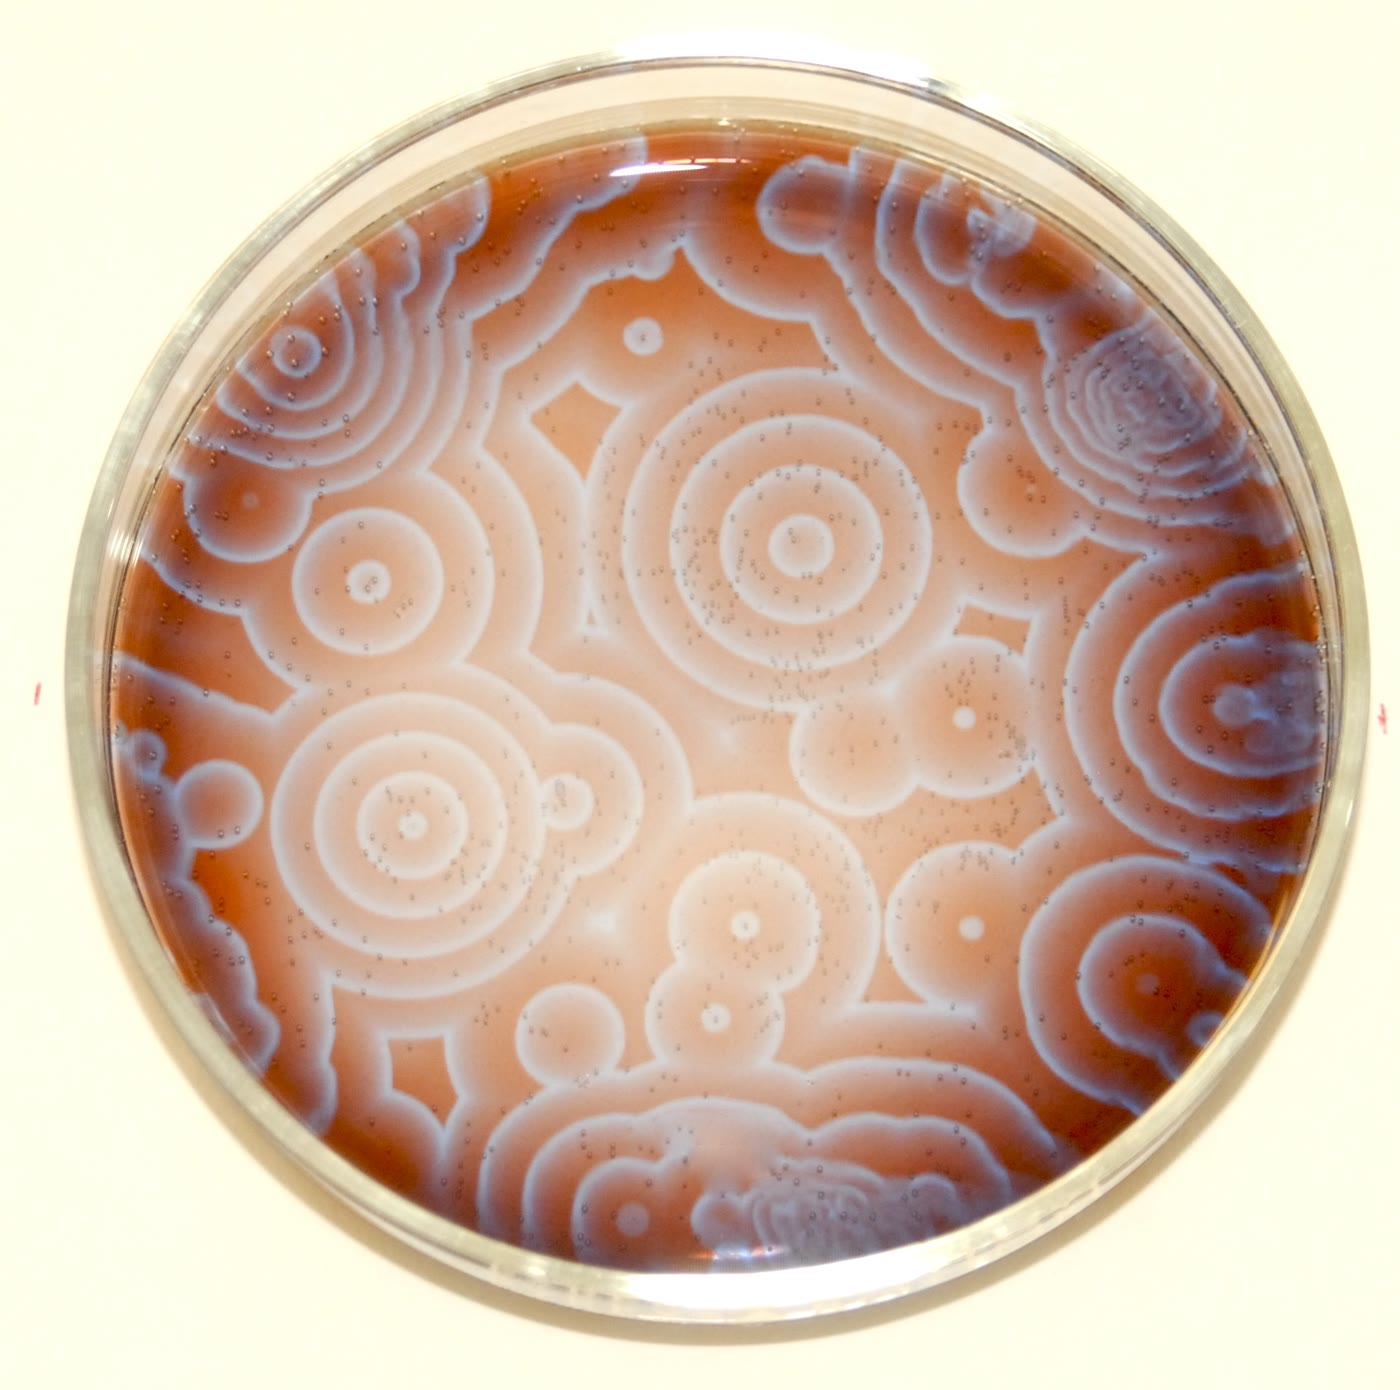
\includegraphics[width=0.48\linewidth]{images/book4/bz-reaction.jpg}

{\small Ondes spirales de la réaction de Belousov--Zhabotinsky dans une
couche mince de solution~: chaque front bleu est une onde d'oxydation du
catalyseur, qui progresse dans le milieu réduit (rouge) et ne peut pas
rentrer dans la région qu'elle vient de quitter.}
\end{omfigure}

\begin{definition}[Méthode de relaxation, temps de relaxation chimique]\label{def:b3:complex-kinetics:relaxation}
Une \emph{méthode de relaxation}\index{methode de relaxation@méthode de relaxation} perturbe
brusquement un système à l'équilibre (par un saut de température, de
pression ou de champ électrique) et suit son retour vers le nouvel
équilibre. Pour une petite perturbation, l'écart décroît
exponentiellement, avec le \emph{temps de relaxation
chimique}\index{temps de relaxation chimique} $\tau$.
\end{definition}

\begin{proposition}[Temps de relaxation d'une association]\label{prop:b3:complex-kinetics:relaxation-time}
Pour $\mathrm{A + B \rightleftharpoons C}$ ($k_1$, $k_{-1}$), après une petite perturbation,
\[
  \frac1\tau = k_1([\mathrm A]_e + [\mathrm B]_e) + k_{-1} .
\]
\end{proposition}

\begin{proof}
Posons $[\mathrm C] = [\mathrm C]_e + x$, $[\mathrm A] = [\mathrm A]_e - x$, $[\mathrm B] = [\mathrm B]_e - x$. Alors $\dot x =
k_1([\mathrm A]_e - x)([\mathrm B]_e - x) - k_{-1}([\mathrm C]_e + x)$~;
les termes sans $x$ se compensent à
l'équilibre, et en négligeant $x^2$~: $\dot x = -[k_1([\mathrm A]_e + [\mathrm B]_e) + k_{-1}]x$.
\end{proof}

La mesure de $\tau$ à plusieurs concentrations donne une droite de
$1/\tau$ en fonction de $[\mathrm A]_e +
[\mathrm B]_e$ dont la pente est $k_1$ et l'ordonnée à l'origine
$k_{-1}$~: les deux constantes, tirées d'expériences sur un système qui
ne s'écarte jamais de l'équilibre de plus de quelques pour cent. Manfred
Eigen mesura ainsi les réactions les plus rapides en solution, dont la
neutralisation de \ce{H3O+} par \ce{OH-}.

\begin{omfigure}
\begin{tikzpicture}
\begin{axis}[width=0.62\linewidth, height=5.0cm, xmin=0, xmax=780, ymin=0, ymax=1.05,
  axis lines=left, xlabel={$t$ / \unit{\micro s}}, ylabel={$([\mathrm C] - [\mathrm C]_e)/([\mathrm C]_0 - [\mathrm C]_e)$},
  tick label style={font=\small}, label style={font=\small},
  legend style={font=\scriptsize, draw=none, at={(0.97,0.97)}, anchor=north east},
  legend cell align=left]
\addplot[omDef, very thick] table[x=t_us, y=dC] {figdata/out/bachelor-3-chemical-relaxation.dat};
\addplot[omThm, thick, dashed] table[x=t_us, y=exp] {figdata/out/bachelor-3-chemical-relaxation.dat};
\legend{équation de vitesse complète, {$\eu^{-t/\tau}$, $\tau = \qty{156}{\micro s}$}}
\draw[black!40, densely dotted] (axis cs:156,0) -- (axis cs:156,0.368) -- (axis cs:0,0.368);
\end{axis}
\end{tikzpicture}

{\small Relaxation de $\mathrm{A + B \rightleftharpoons C}$ après un saut
de température qui a abaissé sa constante d'équilibre de 5\,\% (modèle~:
$k_1 = \qty{1.0e8}{L.mol^{-1}.s^{-1}}$, $k_{-1} = \qty{1.0e3}{s^{-1}}$,
\qty{1.0e-4}{mol/L} de A et de B au total)~: l'équation de vitesse
complète et l'exponentielle de constante
$1/\tau = k_1([\mathrm A]_e + [\mathrm B]_e) + k_{-1}$ coïncident.}
\end{omfigure}

\begin{definition}[Flux stoppé, photolyse éclair]\label{def:b3:complex-kinetics:fast}
La \emph{méthode du flux stoppé}\index{methode du flux stoppe@méthode du flux stoppé} mélange deux
solutions de réactifs en une milliseconde environ en les poussant à
travers un mélangeur jusqu'à une cellule d'observation, puis arrête
l'écoulement et enregistre l'absorbance ou la \omterm{def:b3:electronic-spectroscopy:luminescence}{fluorescence}. La
\emph{photolyse éclair}\index{photolyse eclair@photolyse éclair} crée
une espèce réactive par une impulsion lumineuse brève et intense, et suit
ses réactions à l'aide d'un second faisceau lumineux retardé.
\end{definition}

\begin{omfigure}
\begin{tikzpicture}[font=\small, >=Stealth]
  % two drive syringes
  \foreach \y/\lab in {1.1/A, -0.1/B}{
    \draw[thick] (0,\y) rectangle (2.2,\y+0.6);
    \fill[omDef!25] (0.6,\y+0.05) rectangle (2.15,\y+0.55);
    \draw[thick] (0.6,\y) -- (0.6,\y+0.6);
    \draw[thick] (-0.6,\y+0.3) -- (0.6,\y+0.3);
    \node at (1.4,\y+0.3) {\lab};
    \draw[thick] (2.2,\y+0.3) -- (2.8,\y+0.3);}
  \draw[thick] (2.8,1.4) -- (3.2,0.8) (2.8,0.2) -- (3.2,0.8);
  \node[draw, thick, circle, minimum size=5mm, fill=white] (mx) at (3.4,0.8) {};
  \node[font=\scriptsize, anchor=north west] at (3.22,0.5) {mélangeur};
  \draw[thick] (mx.east) -- (4.4,0.8);
  \draw[thick, fill=omThm!15] (4.4,0.55) rectangle (5.4,1.05);
  \node[font=\scriptsize, anchor=north west, align=left] at (5.0,0.5) {cellule\\ d'observation};
  \draw[->, omThm, thick] (4.9,2.0) -- (4.9,1.1) node[pos=0, above, font=\scriptsize] {lumière};
  \draw[->, omThm, thick] (4.9,0.5) -- (4.9,-0.4) node[below, font=\scriptsize] {détecteur};
  \draw[thick] (5.4,0.8) -- (6.2,0.8);
  \draw[thick] (6.2,0.5) rectangle (7.6,1.1);
  \draw[thick] (7.0,0.5) -- (7.0,1.1);
  \draw[thick] (7.0,0.8) -- (7.9,0.8);
  \draw[thick] (7.9,0.4) -- (7.9,1.2);
  \node[font=\scriptsize, anchor=south] at (6.9,1.15) {seringue d'arrêt};
  \draw[->, black!60] (-1.2,1.4) -- (-0.7,1.4) node[pos=0, left, font=\scriptsize] {poussée};
  \draw[->, black!60] (-1.2,0.2) -- (-0.7,0.2);
\end{tikzpicture}

{\small Un appareil à flux stoppé. Le poussoir entraîne deux seringues~;
les solutions se rencontrent dans le mélangeur et remplissent la cellule
d'observation en une milliseconde environ~; le piston de la seringue
d'arrêt heurte une butée, l'écoulement s'arrête, et le détecteur
enregistre la réaction de la solution fraîchement mélangée.}
\end{omfigure}

\begin{omfigure}
\begin{tikzpicture}
\begin{axis}[width=0.62\linewidth, height=5.0cm, xmin=0, xmax=20, ymin=0, ymax=5.5,
  axis lines=left, xlabel={$t$ / ms}, ylabel={$[\mathrm P_1]$ / \unit{\micro M}},
  tick label style={font=\small}, label style={font=\small}]
\addplot[omDef, very thick] table[x=t_ms, y=P_uM] {figdata/out/bachelor-3-michaelis-menten-burst.dat};
\addplot[black!45, dashed, domain=0:20] {1.28 + 0.2*x};
\draw[->, black!60] (axis cs:4.5,0.7) -- (axis cs:0.25,1.24);
\node[font=\scriptsize, anchor=west] at (axis cs:4.5,0.7) {amplitude de la bouffée, \qty{1.28}{\micro M}};
\end{axis}
\end{tikzpicture}

{\small Un enregistrement de bouffée en flux stoppé (données du problème
du week-end)~: le premier produit d'une \omterm{def:b3:complex-kinetics:enzyme}{enzyme} à deux étapes apparaît en
une bouffée rapide suivie d'une droite~; le trait en tirets extrapole
le régime stationnaire jusqu'à $t = 0$.}
\end{omfigure}

\begin{inthelab}[Une mesure en flux stoppé]
Les deux seringues sont remplies des solutions d'\omterm{def:b3:complex-kinetics:enzyme}{enzyme} et de substrat
dans le même tampon, thermostatées, et actionnées plusieurs fois pour
rincer la cellule avant les tirs enregistrés~; chaque courbe est une
moyenne de cinq à dix tirs. Le temps mort, âge du mélange au début de
l'observation, est mesuré une fois pour toutes avec une réaction de
vitesse connue.
\end{inthelab}

\begin{safety}{\ghs[0.8cm]{GHS05}\ghs[0.8cm]{GHS06}\ghs[0.8cm]{GHS09}}
% ledger: ghs4:Br2
Dibrome~: liquide volatil, dense, rouge-brun~; mortel par inhalation,
provoque de graves brûlures, très toxique pour les organismes
aquatiques. Manipulé uniquement sous hotte, avec des gants et une
protection du visage~; une solution de thiosulfate de sodium est gardée à
portée de main pour réduire les déversements.
\end{safety}

\begin{history}[Bodenstein et Belousov]
Max Bodenstein et Samuel Lind mesurèrent la loi de vitesse de la réaction
dihydrogène--dibrome en 1906~; Jens Christiansen, Karl Herzfeld et
Michael Polanyi l'expliquèrent en 1919 par le mécanisme en chaîne de ce
chapitre. Boris Belousov, biochimiste à Moscou, découvrit sa \omterm{def:b3:complex-kinetics:oscillating}{réaction
oscillante} vers 1951 en cherchant un modèle chimique d'un cycle
métabolique~; son manuscrit fut refusé, et seul un bref résumé parut en
1959. Anatol Zhabotinsky reprit la réaction dans les années 1960 et
l'expliqua~; le mécanisme complet fut établi au début des années 1970.
\end{history}

\section{Exercices}

\begin{exercise}[$\star$]\label{exo:b3:complex-kinetics:1}
Pour la chaîne $\ce{Cl2 -> 2 Cl}$, $\ce{Cl + H2 -> HCl + H}$, $\ce{H + Cl2 -> HCl + Cl}$, $\ce{2 Cl -> Cl2}$,
nommer chaque étape et les \omterm{def:b3:complex-kinetics:chain}{porteurs de chaîne}, et écrire la réaction
globale.
\end{exercise}

\begin{exercise}[$\star$]\label{exo:b3:complex-kinetics:2}
Un système de Lindemann a $k_2 = \qty{1.0e7}{s^{-1}}$ et $k_{-1} = \qty{1.0e10}{L.mol^{-1}.s^{-1}}$
(données de l'exercice). Calculer $[\mathrm M]_{1/2}$ et la pression
correspondante à \qty{750}{K}.
\end{exercise}

\begin{exercise}[$\star$]\label{exo:b3:complex-kinetics:3}
Exprimer $v/V_{\max}$ pour $[\mathrm S] = K_M$, $3K_M$ et $9K_M$. Quelle
concentration donne 90\,\% de
$V_{\max}$~?
\end{exercise}

\begin{exercise}[$\star$]\label{exo:b3:complex-kinetics:4}
% ledger: enz:median.kcatKM, visc:H2O.25C
Une \omterm{def:b3:complex-kinetics:enzyme}{enzyme} a $k_{\mathrm{cat}} = \qty{100}{s^{-1}}$ et $K_M = \qty{0.80}{mM}$.
Calculer sa \omterm{def:b3:complex-kinetics:michaelis}{constante de spécificité} et la comparer à la limite de
diffusion dans l'eau, \qty{7.4e9}{L.mol^{-1}.s^{-1}},
ainsi qu'à la valeur typique de $10^5$~\unit{L.mol^{-1}.s^{-1}}.
\end{exercise}

\begin{exercise}[$\star\star$]\label{exo:b3:complex-kinetics:5}
On propose que la décomposition $\ce{CH3CHO -> CH4 + CO}$ se déroule
ainsi~: $\ce{CH3CHO -> CH3 +
CHO}$ ($k_1$)~; $\ce{CH3 + CH3CHO -> CH4 + CH3CO}$ ($k_2$)~; $\ce{CH3CO -> CH3 + CO}$ ($k_3$)~;
$\ce{2 CH3 -> C2H6}$ ($k_4$). Montrer que la vitesse de formation du
méthane vaut
$k_2(k_1/2k_4)^{1/2}[\ce{CH3CHO}]^{3/2}$.
\end{exercise}

\begin{exercise}[$\star\star$]\label{exo:b3:complex-kinetics:6}
En partant de concentrations égales en \ce{H2} et en \ce{Br2}, avec
$k' = 0.10$, de quel facteur la vitesse a-t-elle diminué quand la
moitié du dibrome est consommée~? Quelle part de cette diminution est
due à l'inhibition~?
\end{exercise}

\begin{exercise}[$\star\star$]\label{exo:b3:complex-kinetics:7}
Dans un mélange modèle dihydrogène--dioxygène (données de l'exercice),
la ramification a la constante de vitesse $f = 1000\,p$, la rupture aux
parois $6000/p$ et la rupture à trois corps
$10\,p^2$, toutes en \unit{s^{-1}} avec $p$ en kPa. Trouver le domaine de
pression dans lequel le mélange explose.
\end{exercise}

\begin{exercise}[$\star\star$]\label{exo:b3:complex-kinetics:8}
Les vitesses initiales valent $\qty{0.20}{\micro M.s^{-1}}$ pour $[\mathrm S] = \qty{0.50}{mM}$ et $\qty{0.40}{\micro M.s^{-1}}$ pour
\qty{2.0}{mM}. Trouver $K_M$ et $V_{\max}$.
\end{exercise}

\begin{exercise}[$\star\star$]\label{exo:b3:complex-kinetics:9}
Avec \qty{50}{\micro M} d'un inhibiteur, la droite de Lineweaver--Burk
d'une \omterm{def:b3:complex-kinetics:enzyme}{enzyme}
($K_M = \qty{0.80}{mM}$) coupe la droite sans inhibiteur sur l'axe des
$1/v$ et coupe l'axe des
$1/[\mathrm S]$ en \qty{-0.417}{mM^{-1}}. Identifier le type d'inhibition
et calculer $K_i$.
\end{exercise}

\begin{exercise}[$\star\star\star$]\label{exo:b3:complex-kinetics:10}
Pour $\mathrm{A + X \to 2\,X}$ avec $k = \qty{0.50}{L.mol^{-1}.s^{-1}}$, $a_0 = \qty{1.00}{mol/L}$ et $x_0 = \qty{0.010}{mol/L}$,
calculer l'instant où la moitié de la quantité finale de X est présente,
et l'instant où la vitesse est maximale.
\end{exercise}

\begin{exercise}[$\star\star\star$]\label{exo:b3:complex-kinetics:11}
Pour le bruxellateur avec $A = 1$, calculer les \omterm{def:b3:quantum-model-systems:operator}{valeurs propres} de la
jacobienne à l'état stationnaire pour $B = 1.5$ et $B = 2.5$, et décrire
le comportement au voisinage de l'état stationnaire dans chaque cas.
\end{exercise}

\begin{exercise}[$\star\star\star$]\label{exo:b3:complex-kinetics:12}
Pour $\mathrm{A + B \rightleftharpoons C}$ avec $k_1 = \qty{1.0e8}{L.mol^{-1}.s^{-1}}$ et $k_{-1} = \qty{1.0e3}{s^{-1}}$, et
$[\mathrm A]_e = [\mathrm B]_e = \qty{2.70e-5}{mol/L}$, calculer $\tau$.
Comment obtiendrait-on les deux constantes de vitesse à partir des seules
mesures de relaxation~?
\end{exercise}

\section{Problème~: une enzyme, un inhibiteur et une dose}

\begin{problem}[{Problème du week-end --- une enzyme, un inhibiteur et
une dose~: les paramètres de Michaelis--Menten par moindres carrés, la
constante d'inhibition d'un inhibiteur compétitif, l'activité restante à
une dose donnée, et une bouffée en flux stoppé}]
\label{pb:b3:complex-kinetics:1}
% ledger: enz:median.kcatKM
Une \omterm{def:b3:complex-kinetics:enzyme}{enzyme} ($[\mathrm E]_0 = \qty{5.0}{nM}$ dans les essais) hydrolyse
son substrat~; vitesses initiales
(données du problème)~:
\begin{center}\small
\begin{tabular}{lccccccc}
\hline
$[\mathrm S]$ / mM & 0.10 & 0.20 & 0.40 & 0.80 & 1.60 & 3.20 & 6.40 \\
$v$ / \unit{\micro M.s^{-1}} & 0.0566 & 0.0981 & 0.169 & 0.247 & 0.340 & 0.397 & 0.447 \\ \hline
\end{tabular}
\end{center}
En présence d'un inhibiteur, des ajustements du même type donnent
$V_{\max}$ inchangée et
la constante $K_M$ apparente~: 0.79, 1.47, 2.38 et \qty{4.02}{mM} pour
$[\mathrm I] = 0$, 20, 50 et
\qty{100}{\micro M}. Une expérience en flux stoppé avec
$[\mathrm E]_0 = \qty{2.0}{\micro M}$ et un substrat saturant
donne l'enregistrement de bouffée de la figure de la section 5 (une
bouffée de \qty{1.28}{\micro M}
de constante de vitesse \qty{625}{s^{-1}}, puis \qty{200}{\micro M.s^{-1}}).

\medskip\noindent\textbf{Partie I --- $K_M$ et $V_{\max}$.}
\begin{enumerate}
  \item Pourquoi utilise-t-on des vitesses initiales~?
  \item Tracer le diagramme de Lineweaver--Burk~; sa droite des moindres
        carrés donne $K_M =
        \qty{0.773}{mM}$ et $V_{\max} = \qty{0.491}{\micro M.s^{-1}}$.
        Quels points la dominent~?
  \item Pourquoi préfère-t-on un ajustement non linéaire direct~?
  \item L'ajustement non linéaire donne $K_M = 0.801 \pm \qty{0.023}{mM}$ et $V_{\max} = 0.502 \pm
        \qty{0.005}{\micro M.s^{-1}}$. Les valeurs de Lineweaver--Burk
        sont-elles compatibles avec elles~?
  \item Calculer $k_{\mathrm{cat}}$.
  \item Calculer la \omterm{def:b3:complex-kinetics:michaelis}{constante de spécificité}.
  \item La comparer à la limite de diffusion et à une \omterm{def:b3:complex-kinetics:enzyme}{enzyme} typique.
\end{enumerate}

\medskip\noindent\textbf{Partie II --- L'inhibiteur.}
\begin{enumerate}[resume]
  \item Quel type d'inhibition les données montrent-elles~?
  \item Écrire $K_M^{\mathrm{app}}$ en fonction de $[\mathrm I]$.
  \item La droite des moindres carrés de $K_M^{\mathrm{app}}$ en fonction
        de $[\mathrm I]$ a pour ordonnée à l'origine \qty{0.799}{mM} et
        pour pente \qty{0.0321}{mM.\micro M^{-1}}. En déduire $K_i$.
  \item Son écart-type vaut \qty{0.9}{\micro M}. Donner un intervalle à
        95\,\% ($t = 4.30$ pour
        deux degrés de liberté).
  \item Que mesure $K_i$~?
\end{enumerate}

\medskip\noindent\textbf{Partie III --- L'activité restante.}
\begin{enumerate}[resume]
  \item Exprimer la fraction d'activité restante, $v_i/v_0$, en fonction
        de $[\mathrm S]$ et de
        $[\mathrm I]$.
  \item L'évaluer pour $[\mathrm S] = K_M$ et $[\mathrm I] = K_i$.
  \item Pour $[\mathrm S] = K_M$ et $[\mathrm I] = 10K_i$.
  \item Pour $[\mathrm S] = 10K_M$ et $[\mathrm I] = 10K_i$. Commenter.
  \item Montrer qu'une inhibition à 90\,\% pour $[\mathrm S] = K_M$ exige
        $[\mathrm I] = 18K_i$.
  \item Calculer cette concentration avec le $K_i$ ajusté.
\end{enumerate}

\medskip\noindent\textbf{Partie IV --- La bouffée.}
\begin{enumerate}[resume]
  \item L'\omterm{def:b3:complex-kinetics:enzyme}{enzyme} fonctionne en deux étapes, $\mathrm{E + S \to E{-}acyl + P_1}$ ($k_2$) puis $\mathrm{E{-}acyl \to E +
        P_2}$ ($k_3$). Pourquoi $\mathrm P_1$ apparaît-il en une
        bouffée~?
  \item L'amplitude de la bouffée vaut $[\mathrm E]_0\bigl(k_2/(k_2 + k_3)\bigr)^2$.
        En déduire $k_2/(k_2 + k_3)$.
  \item À partir de la pente du régime stationnaire, calculer
        $k_{\mathrm{cat}}$ et le comparer à la partie I.
  \item La constante de vitesse de la bouffée vaut $k_2 + k_3$. En
        déduire $k_2$ et $k_3$.
  \item Vérifier que $k_{\mathrm{cat}} = k_2k_3/(k_2 + k_3)$.
  \item Énoncer le résultat~: la concentration d'inhibiteur qui donne une
        inhibition à 90\,\% pour
        $[\mathrm S] = K_M$.
\end{enumerate}
\end{problem}
